% Some notation taken from 
% https://cs230.stanford.edu/files/Notation.pdf

% On variables, parameters, and arguments
% https://math.stackexchange.com/questions/2113138/what-is-the-difference-between-variable-argument-and-parameter

\documentclass{article}
\usepackage[sorting=none]{biblatex}
\addbibresource{sources.bib}

%Graphics: https://www.overleaf.com/learn/latex/Inserting_Images
\usepackage{graphicx}
\graphicspath{{figures/}}

% https://tex.stackexchange.com/questions/2651/should-i-use-center-or-centering-for-figures-and-tables
\makeatletter
\g@addto@macro\@floatboxreset\centering
\makeatother

% https://tex.stackexchange.com/questions/268766/curly-braces-in-math-mode
\usepackage{mathtools}
\DeclarePairedDelimiter\set\{\}

% https://github.com/battlesnake/neural
% \usepackage{neuralnetwork}

\usepackage{amsmath}

% https://tex.stackexchange.com/questions/286094/insert-code-keywords-inline
\usepackage{xcolor}
% \usepackage{listings}
% \lstset{language=Python, keywordstyle=\bfseries \color{blue}}
\usepackage{xparse}
\NewDocumentCommand{\codeword}{v}{%
\texttt{\textcolor{blue}{#1}}%
}

% Titular information
% https://en.wikibooks.org/wiki/LaTeX/Title_Creation
\title{
	An Undergraduate's Explanation of the Multilayer Perceptron: 
	Mathematical Concepts and a Python3 Implementation}
\date{2022 \\ January}
\author{Jared Frazier\thanks{Department of Computer Science (2021-2022), 
Middle Tennessee State University.} \thanks{Not endorsed by or affiliated with any of the 
authors or entities associated with references.}}
\begin{document}
\maketitle

\section{Preamble}
\quad The purpose of the present document is to explain and implement the major mathematical
constructs/concepts behind feedforward neural networks, specifically the multilayer perceptron.
This includes the layers that compose such networks, the cost (aka loss, error, or objective) function
and activation functions, the forward pass through the network,
the computation of gradients via backpropagation (a concept that is often "handwaved" to the extreme
or explained in so much detail as to be utterly confusing--at least my experience),
and the update of model parameters via mini-batch stochastic gradient descent.
If the ideas such as \textit{layer} and \textit{backpropagation} are entirely unfamiliar
to you, then I encourage you to visit 3Blue1Brown's Deep Learning YouTube Series \cite{3Blue1BrownWhatIsANN2017}
and peruse the first few chapters of texts such as \textit{Deep Learning} (free, online) \cite{Goodfellow2016},
\textit{Neural Networks and Deep Learning} (free, online) \cite{Nielsen2015},
\textit{Hands-on Machine Learning with Scikit-Learn, TensorFlow and Keras 2ed} (buy) \cite{Geron2020},
and/or \textit{Deep Learning with Python 2ed} (buy) \cite{Chollet2021}. The present document
is not intended to be a comprehensive overview of neural networks nor an extremely
in-depth mathematical treatise but rather a document that highlights certain concepts that the
author found confusing or ambiguous when he was learning about neural networks
(particularly regarding the backpropagation algorithm).

\section{Introduction}

\quad The neural network (function approximator) is just a chain of geometric transformations (functions)
each parametrized by a weight matrix $W \in \mathcal{R}^{n_h \times n_x}$ and
a bias vector $b \in \mathcal{R}^{n_h}$ on the input vector $x \in \mathcal{R}^{n_x}$.
The geometric transformations of the neural network are encapsulated by connecting
layers (e.g., dense/fully connected layers) together. A neural network has $L$ total
layers and the current layer $l$ receives the output from the previous layer $(l-1)$.
Note that $n_x$ is the number of features (or independent variables) in the input
and $n_h$ is the number of hidden units in the current layer. The following subsections will
breifly elucidate the claims in of the first setnence of this section and the
corresponding notation.

\subsection{Parametrized Functions}

The author assumes you know what a function is; however, the term \textit{parametrized}
is one that appears often in deep learning literature and should be well-understood by the student.
Consider a generic quadratic function \cite{MathSEVarsParamsArgs2015} as
% Quadratic function
\begin{equation}
	f(x) = ax^{2} + bx + c
\end{equation}
The \textit{variable} $x$ is an \textit{argument} to the function $f$ that has
\textit{parameters} $a$, $b$, and $c$. The parameters determine the behavior of
the function (e.g., the steepness of slope, intercepts, shape, etc.) while the
variable can take on some range of values. When a variable that takes on a particular
value is passed as an argument to the function with defined parameters, the result
is some other value $y$ if $y = f(x)$. This explanation of a function
should not be anything new; however, the \textit{parameters} are quantities
of particular interest for neural networks since the parameters are the quantities
that are \textit{learned} by the neural network over time. What it means to learn
parameters will be explaned later.

A neural network can be denoted as a function $h$ with parameters $W$
and $b$ of a variable $x$. This statement can be compactly written as
$h_{W, b}(x)$. The subscript with $W$ and $b$
means that the weights $W$ and biases $b$ are parameters of the neural network $h$.
The claim that a neural network is a chain of functions is useful later during
the updating of the parameters of the network. But to briefly illustrate the idea
of chaining functions, the generic quadratic function in Equation 1 is decomposed
into units called \textit{atomic functions}.
\begin{align}
	g_{a}(x)     & = ax^{2}                  \\
	u_{b}(x)     & = bx                      \\
	f_{a,b,c}(x) & = g_{a}(x) + u_{b}(x) + c
\end{align}
Decomposing functions into their constituent atomic functions is useful
for applying rules of calculus--the basis of parameter learning via
the backpropagation algorithm illustrated later.

\subsection{Operand Types}

The input $x$ is not a single value as is conceived in the elementary
formulations described above. Rather, the input $x$ is a list of
values referred to as a \textit{column vector}. Each element of the vector
is a value that a particular feature, or independent variable, could take on.
The shape of the vector $x$ is important to understand since the functions and operations
performed by the neural network (dot product, Hadamard product, addition, etc.)
restrict their vector/matrix operands to particular shapes. When using the term
\textit{vector}, I am always referring to a \textit{column vector}
unless otherwise specified. Also, note that $x \in \mathcal{R}^{n_x}$ indicates
that $x$ is a vector with $n_x$ elements and the $j^{th}$ is a real number.
For example, the below vector $x$ is shown and a common vector operation
known as transposition (converts a \textit{column vector} to a
\textit{row vector} and is denoted with a superscript of $\top$) is also shown.
\begin{align}
	x & = \begin{bmatrix}
		x_{1}  \\
		x_{2}  \\
		x_{3}  \\
		\vdots \\
		x_{(n_x)}
	\end{bmatrix}
	=
	\begin{bmatrix}
		x_{0}  \\
		x_{1}  \\
		x_{2}  \\
		\vdots \\
		x_{(n_{x}-1)}
	\end{bmatrix}
	=
	\begin{bmatrix}
		x_{0} & x_{1} & x_{2} & \cdots & x_{(n_{x}-1)}
	\end{bmatrix}^\top
\end{align}

Many programming languages assign the first element of a vector the index
0; this notation is shown above in addition to the more standard
mathematical notation where the first element begins with the index 1.
For the remainder of this document, I will use the index 0 assumption
since my implementation of the neural network uses the Python
programming language. If you wish to implement the same algorithms in a language
such as R or Wolfram Mathematica, be wary of this index discrepancy.
Consequently, with index beginning at 0, the last index of a vector with
$n_x$ elements will be $(n_x - 1)$... and woe is the programmer who commits an
off-by-one error.

Lastly, a matrix $W$ represents the weight of edges between the $k^{th}$
input neuron of $n_x$ total input neurons (i.e., neurons in the previous layer)
and the $j^{th}$ hidden neuron of $n_h^{l}$ total hidden neurons.
A weight matrix looks similar to the vector, except rather than having a single
column, a matrix has a rows and columns--looking like a table. Vectors can
be referred to as rank-1 tensors, matrices as rank-2 tensors, so and so forth
for multiple index "lists" in higher dimensions. A sample weight matrix
$W \in \mathcal{R}^{n_h \times n_x}$ is
shown below.

\begin{align}
	\begin{bmatrix}
		W_{00}         & W_{01}         & W_{02}         & \cdots & W_{0(n_{x}-1)}         \\
		\vdots         & \vdots         & \vdots         & \vdots & \vdots                 \\
		W_{(n_{h}-1)0} & W_{(n_{h}-1)1} & W_{(n_{h}-1)2} & \cdots & W_{(n_{h}-1)(n_{x}-1)}
	\end{bmatrix}
\end{align}

\section{The Multilayer Perceptron}
\quad Here I define the operations that occur for a multilayer perceptron (MLP).
Note that the MLP can sometimes refer to any class of feedforward
neural network, that is a network that applies affine transformations and
activation functions to input from a previous layer in the network.

\subsection{The Dense/Fully Connected Layer}
The affine transformation, which is the most fundamental transformation
of the densely/fully connected layers that exist in the MLP, yields
a weighted input vector $z^{l}$ with elements
$z_j^{l} = W_{jk}^{l} a_{k}^{l-1} + b_{j}^{l}$ for a layer $l$ and neuron $j$.
Here, the activation $a_k^{l-1}$ denotes the activation of the $k^{th}$ neuron of the
previous layer $(l-1)$. Importantly, the input layer has no activation function $\phi$
associated with it, so the activation vector $a^{0}$ equals the input vector $x$.
Moreover, the inner dimensions of the matrix product
$Wx$ match, that is the subscripts $k$ are "adjacent" to one another. While you may
observe that the activation vector $a \in \mathcal{R}^{n_a}$ is clearly not a matrix,
numerical libraries will often treat a vector $v \in \mathcal{R}^{n_v}$ as equivalent
to a matrix with a single column (i.e., $V \in \mathcal{R}^{n_v \times 1}$) for
the purposes of performing fast matrix-matrix calculations.

Until now the discussion of the MLP has been entirely in abstract mathematical
notation, so now a visual of a single layer (meaning single hidden layer)
MLP is shown. The activation function $\phi$ is vectorized, meaning it
applies to each element of a vector, matrix, or rank-n tensor. The number of
neurons in a hidden layer (or output layer for that matter) $n_h$ does not have
to be constant, and this is shown in the figure below where the output layer
has only a single neuron while the hidden layer has three neurons.

% Multilayer perceptron figure
\begin{figure}[h]
	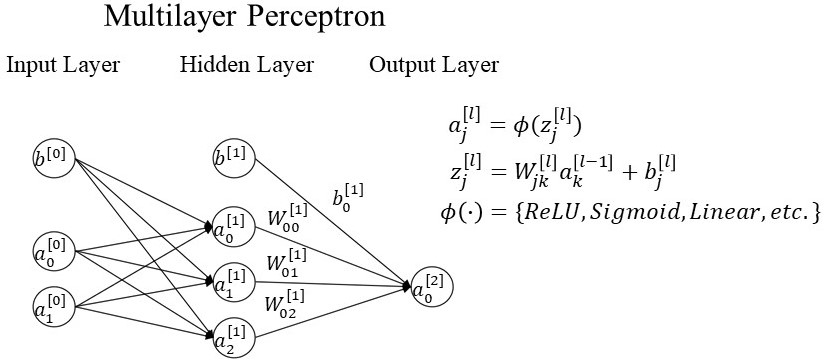
\includegraphics[scale=0.60]{mlp_larger_font_croppped.jpg}
\end{figure}

% Multilayer percetpron with useneuralnetwork pkg
% \begin{align}
% 	\begin{neuralnetwork}[height=3, layertitleheight=5.0em]
% 		\newcommand{\x}[2]{$a^{0}_#2$}
% 		\newcommand{\hfirst}[2]{\small $a^{(1)}_#2$}
% 		\newcommand{\y}[2]{$a^{2}_#2$}
% 		\inputlayer[count=2, bias=false, title=Input Layer 0, text=\x, nodeclass={input neuron}]
% 		\hiddenlayer[count=3, bias=false, title=Hidden Layer 1, text=\hfirst, nodeclass={hidden neuron}] \linklayers
% 		\outputlayer[count=1, title=Output Layer 2, text=\y, nodeclass={output neuron}] \linklayers
% 	\end{neuralnetwork}
% \end{align}

% Neural Network Definition
\subsection{The Forward Pass and Cost Function}
\quad The MLP is a function approximator and the MLP learns the parameters of
this function. Since the learning is just the determination of the values of the
parameters of the MLP, then there must be some other function that determines
how well the parameters of the MLP approximate the desired function. This other
function is called the cost or loss function and is denoted C, though sometimes
it will be denoted $\mathcal{L}$. For regression problems, the most common
cost function is the mean squared error. The cost function, unlike previous
operations, returns a scalar and \textit{not} a vector. However, the cost for
a single sample $C_x$ is a vector. The scalar value can be used to estimate
performance during training; however, for my implementation, the cost vector
$C_x$ is used for learning MLP parameters.

\begin{equation}
	\begin{aligned}
		\text{C} & = \frac{1}{N} \sum_{x} {C_x}                   \\
		         & = \frac{1}{N} \sum_{x} {(\hat{y} - y)^{2} }    \\
		         & = \frac{1}{N} \sum_{x} {(h_{W,b}(x) - y)^{2} } \\
		         & = \frac{1}{N} \sum_{x} {(a^{L} - y)^{2} }
	\end{aligned}
\end{equation}

The cost function for a single sample $C_x$ is a multivariable function
and it can also be written as a function of its parameters $\theta$ like
$C_x(\theta)$ where $\forall$ layers $l,\ \theta = \set{W^{l}, b^{l}}$. $C_x$ can
also be written to emphasize a certain parameter such as the weight $C(W)$. More importantly,
the derivative of the cost function with respect to each activation $j$ of
the last layer (i.e., output layer) $L$ is defined as
$\frac{\partial C_x}{\partial a_j^{L}}$ and this is
relevant to the backpropagation algorithm illustrated shortly.

Put simply, The activation vector $a^{L}$ for the last layer $L$ is the prediction
that the MLP makes. The activation $a^{L}$ naturally has some number of elements
determined by the number of units $n_h$ in the layer, and to index the $j^{th}$
activation of the activation vector one would write $a_j^{l}$. The activation for
the $j^{th}$ neuron is used to compute errors that are relevant for the
backpropagation algorithm since how well $a^{L}$ "lines up" with the known
result $y$ is determined by the choice parameters $W$ and $b$ for all layers $l$.

\subsection{Backpropagation}

The key to learning for the MLP, and for artificial neural networks in general,
is updating the weights $W^{l}$ and biases $b^{l}$ for each layer $l$ such
that the network performs better with respect to the loss function.\footnote{
Machine learning APIs like TensorFlow tend to formulate cost functions
such that they can be \textit{minimized} (e.g.,
$minimize(NegativeLogLikelihood) \equiv maximize(LogLikelihood)$)}.
Since $W$ and $b$ are tensors, the gradients\footnote{Remember this is denoted
	using the gradient $\nabla$ or $\vec{\nabla}$ operator.}
of these parameters ($W$, $b$) with respect to each variable (e.g.,
$\frac{\partial C_x}{\partial W_{jk}^{l}}$ or
$\frac{\partial C_x}{\partial b_{j}^{l}}$) in the parameter matrix or vector.

At this point you might ask yourself again what the difference between
variables and parameters is. In pure mathematics classes, you are often asked
to minimize a function with respect to some variable(s), and rarely (at least in
my experience) with respect to a parameter. Why minimize the cost
function with respect to the parameters? The statement "minimize with respect
to a parameter" seemed to contradict the very definition of a parameter:
"argument that are... not explicitly varied in situations of interest are termed
\textit{parameters}" \cite{WolframMathWorldParameterDefinition}. The simplest
answer I can surmise is that the parameters are constant for a single iteration
of a machine learning experiment, and then updated such that the model performs
better on future experiments. An experiment here encompasses the fitting of a
model for a number of iterations equal to
$NumEpochs \times frac{TrainingDataSize}{BatchSize}$. A "batch" for learning
is just a random subset of size $m$ of the training data and thus, one iteration of the
machine learning experiment is performing the forward pass, computing the gradients
for the weight matrices and biases of each layer, and then updating those
parameters. Parameters are intrinsic to the model, that mathematical object
that maps input to some desired output, while variables are simply inputs
to the model.

Knowing that the parameters need to be updated, most often the below equations
will be written and the gradient computation process might be abstracted from
the reader. The equations make quite a lot of sense if you think about exactly
what they are saying. The first of the three equations says "update the
weight matrix for a given layer by subtracting from the current weight matrix
computing the cost function with respect to that same weight matrix." By definition,
the gradient "points" in the direction of local maxima [\textbf{CITATION}], so
negative gradient points in the direction of local minima. The "step size" of
such an update is proportional to the leraning rate $\eta$, which is a
hyperparameter (a parameter explicitly set by a user) of the model.

\begin{align}
	W^{l}      & = W^{l} - \eta \nabla_{W^{l}}C \\
	b^{l}      & = b^{l} - \eta \nabla_{b^{l}}C \\
	\theta^{l} & = \eta \nabla_{\theta^{l}}C
\end{align}

However, the following equations that are critical for gradient descent
are claimed without proof (see \cite{Nielsen2015} for proofs). Note, that while
the previous equations are the "pretty" form of gradient descent, for the
accompanying implementation, one does not compute the gradient directly.

\begin{align}
	\delta^{L}                                    & = \nabla_{a} \text{C} \circ \frac{\partial \phi}{\partial z}(z^{L})             \\
	\delta^{l}                                    & = ((w^{l+1})^{\top} \delta^{l+1}) \circ \frac{\partial \phi}{\partial z}(z^{l}) \\
	\frac{\partial \text{C}}{\partial b_j^{l}}    & = \delta_j^{l}                                                                  \\
	\frac{\partial \text{C}}{\partial W_{jk}^{l}} & = a_{k}^{l-1}\delta_{j}^{l}
\end{align}

The practical implementation of the four equations will be explained shortly
after showing the \textit{gradient descent} equations below.

\begin{align}
	W^{l} & = W^{l} - \frac{\eta}{m} \sum_{x}{\delta^{x, l}(a^{x, l-1})^\top} \\
	b^{l} & = b^{l} - \frac{\eta}{m} \sum_{x}{\delta^{x, l}}
\end{align}

The learning rate $\eta$ is typically $\eta = \set{1^{i}}_{i=-2}^{-4}$, and $m$
for mini-batch stochastic gradient descent is typically
$m = \set{2^{i}}_{i=1}^{10}$.

\section{Implementation}
Here I define, somewhat out of order, the Python \codeword{class}es
that will encapsulate the attributes (data members) and methods associated
with the MLP. Since this approach is object oriented, it was helpful to
define first the subunits of the MLP: operations (such as activation functions)
and layers.

The \textbf{forward pass} requires defining a \codeword{class} that
encapsulates the fully/densely connected layer of the MLP. The author defines this as
\codeword{DenseLayer} with attributes for the input dimensions $n_x$,
the weight matrix $W \in \mathcal{R}^{n_x \times n_h}$, and the bias
$b \in \mathcal{R}^{n_h}$. The \codeword{DenseLayer} is correspondingly passed
arguments for $n_x$, $n_h$, and an optional Python \codeword{Callable}
that will be used as the activation function $\phi$ for a given layer.
The methods for the \codeword{DenseLayer} use Glorot Uniform initialization \cite{Glorot2010}
for the weight matrix and a forward pass is also defined as

\begin{equation}
	ForwardPassResult = \phi(Wx + b)
\end{equation}
where $x$ is an argument to the \codeword{__call__} method of the
\codeword{DenseLayer}.

The \textbf{activation functions and cost functions} are children of the Python
abstract base class I define as \codeword{Operation}. The
\codeword{Operation} has no arguments and initializes no attributes, but
does have a \codeword{__call__} method, \codeword{derivative} method. All
children of the \codeword{Operation} must implement these methods. However, if
the child is a \textit{cost function}, then this child class must also
implement a \codeword{gradient} method ($\nabla_{a}\text{C}$).

\pagebreak
\printbibliography

\end{document}